\documentclass[a4paper,spanish]{article}
\usepackage[activeacute]{babel}
\usepackage[utf8]{inputenc}
\usepackage{listings}
\usepackage{graphicx}
\usepackage{epsfig}
\usepackage[font=small,labelfont=bf]{caption}
\usepackage{hyperref}
\hoffset=-2.5cm
\textwidth=17cm
\parskip=1ex
\usepackage{framed}
\usepackage{escenarios}
\usepackage{riesgos}



%opening
\title{Ingenier\'ia de Software II\\ \textbf{Sistema ``Twitteando para Ahorrar''}}
\author{\textbf{Grupo 6}\\ 1º Cuatrimestre 2013} 
\date{}


\begin{document}

\maketitle
\vspace{10cm}
\begin{center}

\begin{tabular}{|c|c|c|}
\hline
\hline
\textbf{LU}&\textbf{Nombre}&\textbf{email}\\
\hline
667/06&Daniel Foguelman &dfoguelman@dc.uba.ar\\
\hline
767/03&Hern\'an Modrow&hmodrow@gmail.com\\
\hline
511/00&Leonardo Tilli&leotilli@gmail.com\\
\hline
\hline
\end{tabular}
\end{center}
\newpage

\section{Parte I}

 En esta primera parte del informe presentamos la planificaci\'on para el proyecto TPA para las etapas subsiguientes a lo creado en la entrega anterior. En este proceso, integraremos el Core de Twiteando para Ahorrar con m\'ultiples servicios (Redes sociales, detecci\'on de fraude, etc), tendremos requerimientos funcionales y no-funcionales de media y gran complejidad. Esto Nos mueve del paradigma SCRUM por uno m\'as tradicional, RUP, haciendo preponderancia en la planificaci\'on y an\'alisis de requerimientos antes que en la adaptabilidad al cambio y visibilidad del proyecto. \\

 El plan desarrollado para esta nueva etapa sigue el modelo RUP, y se documenta a continuaci\'n. Primero se describir\'an los casos de uso identificados. En base a esto se detallan las distintas iteraciones que se planificaron y de qu\'e consta cada una. En la \'ultima secci\'on se encuentra el an\'alisis de los riesgos m\'as importantes que se detectaron.


\section*{Lista de Casos de Uso}

\section*{Riesgos}

%Template
%\begin{riesgo}{SITUACION}{CONSECUENCIA}
%    \contexto{Texto de contexto}
%    \probabilidad{Baja-Media-Alta}
%    \impacto{Cr\'itico-Medio-Bajo}
%    \exposicion{Alta-Media-Baja}
%    \mitigacion{Texto mitigacion}
%    \contingencia{Texto contingencia}
%\end{riesgo}

\begin{riesgo}{el/los cluster/s armados pueden no tener suficiente poder de computo}{los tiempos de respuesta y el conjunto de datos analizados no sean los esperados.}
    \contexto{Se espera manejar grandes vol\'umenes datos y de peticiones por lo tanto necesita alto poder de procesamiento y una gran cantidad de espacio para almacenarse.}
    \probabilidad{Media}
    \impacto{Alto}
    \exposicion{Alta}
    \mitigacion{Diseñar arquitectura que escale horizontalmente y sea f\'acil agregar capacidad de procesamiento y de datos.}
    \contingencia{Disminuir la cantidad de informaci\'on que se puede recibir y enviar TPA a los usuarios. Analizar la distribuci\'on del sistema en nodos que abarquen las consultas de determinadas regiones.}
\end{riesgo}

\begin{riesgo}{la arquitectura se define con computadores de bajo costo}{se ca\'iga la base de datos con la informaci\'on de las ofertas}
    \contexto{La ca\'ida de la infraestructura de repositorios de ofertas generar\'ia una caida del servicio completo.}
    \probabilidad{Baja}
    \impacto{Alta}
    \exposicion{Media}
    \mitigacion{Informaci\'on guardada con chequeos de integridad que permitan una f\'acil recuperaci\'on (RAID). Redundancia de la base de datos con informaci\'on de la ofertas.}
    \contingencia{Recuperar la informaci\'on utilizando chequeo de integridad de datos. Levantar sistemas de base de datos de backup.}
\end{riesgo}

\begin{riesgo}{el sistema se espera sea usado masivamente}{se genere mucha carga en el uso del sistema que produzca lentitud de respuesta}
    \contexto{Dado que el sistema TPA tendr\'a impacto a nivel nacional y regional, es esperable una gran carga de consultas.}
    \probabilidad{Alta}
    \impacto{Alta}
    \exposicion{Alta}
    \mitigacion{Generar una arquitectura que permita la alta disponibilidad del servicio utilizando \textbf{cach\'es} distribuidos para minimizar la carga en cada servidor. Armar casos de tests espec\'ificos para detectar problemas de disponibilidad en el sistema.}
    \contingencia{Levantar clusters adicionales, en caso de no ser posible evaluar la contrataci\'on de clusters externos.}
\end{riesgo}

\begin{riesgo}{se quiere que el sistema sea usado por la mayor cantidad de gente y en la mayor cantidad de plataformas}{no sea homogeneo entre las distintas plataformas y f\'acil de usar para todos los usuarios}
    \contexto{La aplicaci\'on TPA deber\'a tener alcance nacional y ser inclusiva para todos y todas. Las personas de edad avanzada o con capacidades especiales deber\'an poder utilizar las interfaces de usuario de manera intuitiva.}
    \probabilidad{Bajo}
    \impacto{Bajo}
    \exposicion{Baja}
    \mitigacion{Buscar especialistas en usabilidad para generar interfaces aptas.}
    \contingencia{No hacer nada, el porcentaje de estos usuarios es menor en comparaci\'on a los usuarios activos.}
\end{riesgo}

\begin{riesgo}{los servicios del sistema se proveer\'an a trav\'es de Internet}{recibir un ataque de Denegaci\'on de Servicio (DoS y DDoS) no siendo posible brindar los servicios}
    \contexto{Existen grupos de activistas que con distintas motivaciones atacan sitios mediante ataques de denegaci\'on de servicio para hacer llegar su mensaje. Estos ataques son faciles de generar y ejecutables en todo tipo de computadoras, incluso celulares o tablets, por lo que pueden ser facilmente escables por un grupo coordinado.}
    \probabilidad{Media}
    \impacto{Alta}
    \exposicion{Alta}
    \mitigacion{Generar una aplicaci\'on distribuida con buena distribuci\'on de carga para poder soportar alta carga de datos. Organizar periodicamente simulaciones de este tipo de ataques para probar el sistema. }
    \contingencia{Minimizar el tiempo de reinicializaci\'on de los servicios de TPA. Analizar la distribuci\'on del sistema en nodos que abarquen las consultas de determinadas regiones. Evaluar la contrataci\'on de sistema contra este tipo de ataques.}
\end{riesgo}

\begin{riesgo}{se almacena informaci\'on de los usuarios en sistema}{esa informaci\'on sea robada}
    \contexto{Dada la exposici\'on de los usuarios as\'i como otra informaci\'on que se requiera que sea relevante al sistema, ej: configuraci\'on de confianza, h\'abitos de utilizaci\'on, dicha informaci\'on es suceptible de ser comercializada.}
    \probabilidad{Alta}
    \impacto{Medio}
    \exposicion{Alta}
    \mitigacion{Anonimizar la informaci\'on de los usuarios utilizada internamente. Aislar los datos sensibles de los usuarios de otros partes del sistema, encriptar, restringir y auditar su utilizaci\'on. Realizar simulaciones de ataques para encontrar vulnerabilidades.}
    \contingencia{Cerrar las consultas de informaci\'on y dejar solo accesible las consultas de ofertas generales.}
\end{riesgo}

\begin{riesgo}{el sistema depende en gran parte de la informaci\'on provista por lo usuarios}{haya un alto porcentaje de ofertas dudosas}
    \contexto{Dado que el proyecto es esponsoreado por el gobierno nacional, es posible que un n\'umero importante de ofertas dudosas sean generadas que buscan manipular el sistema en pos de un beneficio personal.}
    \probabilidad{Bajo}
    \impacto{Medio}
    \exposicion{Media}
    \mitigacion{Informar a los usuarios de los beneficios de usar el sistema correctamente. Buscar la adopci\'on temprana del sistema por parte de los usuarios para que estos generen un alto n\'umero de datos. Utilizar los servicios de SpamBuster para el filtrado de ofertas dudosas mientras se genera un m\'odulo proprio. Invalidaci\'on de ofertas manualmente por usuarios administrativos/configuraci\'on.}
    \contingencia{Generar listas de productos oficialmente verificados por agentes de TPA.}
\end{riesgo}

\begin{riesgo}{dado el contexto inflacionario y de polarizaci\'on pol\'itica}{informaci\'on no sea confiada por los usuarios}
    \contexto{La poca credibilidad en los \'indices inflacionarios podr\'ia inducir a la falta de confianza de los usuarios a los resultados de b\'usqueda.}
    \probabilidad{Baja}
    \impacto{Bajo}
    \exposicion{Baja}
    \mitigacion{Generaremos reportes de confianza para entender las necesidades de los usuarios y mejorar la confiabilidad de las ofertas sugeridas.}
    \contingencia{Evaluar la realizaci\'on de una campaña publicitaria para generar confianza en los usuarios. Evaluar la posibilidad de la captura de ofertas mediante fotos.}
\end{riesgo}

\begin{riesgo}{el sistema depende en gran parte de la informaci\'on provista por lo usuarios}{haya un gran n\'umero de usuarios no confiables}
    \contexto{Dado que el proyecto es esponsoreado por el gobierno nacional, es posible que se registren usuarios que hagan busquen el fracaso del sistema, ej: disminuyendo la confiabilidad de las ofertas.}
    \probabilidad{Bajo}
    \impacto{Medio}
    \exposicion{Baja}
    \mitigacion{Generar estrategias de validaci\'on de usuarios para minimizar la falsificaci\'on de identidad. Evaluar la generaci\'on programas de fidelizaci\'on fin de que los usuarios quieran registrarse utilizando informaci\'on fidedigna y participar activamente generando informaci\'on confiable.}
    \contingencia{Los usuarios deber\'an verificarse personalmente para poder utilizar el sistema.}
\end{riesgo}

\begin{riesgo}{el presupuesto es acotado y se espera que el sistema genere ingresos propios a fin de mantenerse}{los fondos obtenidos de los servicios pagos ofrecidos sean insuficientes y el proyecto fracase}
    \contexto{El proyecto depende de fondo.}
    \probabilidad{Baja}
    \impacto{Alto}
    \exposicion{Media}
    \mitigacion{Venta de servicios para sugerir ofertas de comerciantes. Venta de informaci\'on est\'adistica del sistema.}
    \contingencia{Agregar ventea publicadad al sistema. Solicitar fondos adicionales al estado nacional. Buscar fuentes de financiaci\'on adicionales.}
\end{riesgo}

\begin{riesgo}{es necesario obtener informaci\'on de ofertas distintos sistemas/p\'aginas web mediante webcrawling}{no se descubran correctamente las ofertas de los mismos}
    \contexto{La programci\'on de analizadores de leguaje natural es una tarea compleja que requiere un alto nivel de conocmiento para implementarse correctamente.}
    \probabilidad{Media}
    \impacto{Medio}
    \exposicion{Media}
    \mitigacion{Alguno de los miembros del equipo asistar\'a a una capacitaci\'on sobre el tema, para que luego realice capacitaci\'on interna. Implementaremos estrat\'egias de entrenamiento de la plataforma y generaremos m\'ultiples casos de test para verificar la identificaci\'on de ofertas. Tambi\'en utilizaremos una estrategia de supervisi\'on de la identificaci\'on de ofertas por un operario manual a fin de mejorar la detecci\'on.}
    \contingencia{Contrataremos personal que identifique las ofertas que no se est\'an encontrando para poder generar nuevas estrategias de detecci\'on.}
\end{riesgo}

\begin{riesgo}{es necesario almacenar la informaci\'on de las ofertas en un base de datos no relacional (NOSQL) y el equipo tiene poca experiencia}{de que el proyecto se atrase o de que fracase debido al mal armado del modelo de datos}
\contexto{Se solitica la utilizaci\'on de una base de datos no relacional a fin guardar la informaci\'on de las ofertas.}
\probabilidad{Alta}
\impacto{Alto}
\exposicion{Alta}
\mitigacion{Alguno de los miembros del equipo asistar\'a a una capacitaci\'on sobre el tema, para que luego realice capacitaci\'on interna.}
\contingencia{Contratar a un especialista en el tema para que participe del proyecto. Alternativamente tercerizar esa parte del proyecto.}
\end{riesgo}

\begin{riesgo}{se utilizar\'an m\'aquina es necesario armar uno (o varios) clusters y que los miembros delequipo no tienen experiencia en esto}{de que el proyecto se atrase o de que fracase en cuanto al nivel de procesamiento de datos que realiza}
\contexto{Se dispone de PCs comunes para el deploy del sistema. Dado que se requiere un alto nivel de procesamiento es que se deber\'an armar clusters con las PCs a fin de generar mayor poder de computo.}
\probabilidad{Alta}
\impacto{Alto}
\exposicion{Alta}
\mitigacion{Alguno de los miembros del equipo asistar\'a a una capacitaci\'on sobre el tema, para que luego realice capacitaci\'on interna. Destrabar la importaci\'on de los servidores dedicados.}
\contingencia{Contratar a un especialista en el tema para que participe del proyecto. Evaluar la contrataci\'on de un servicio externo de procesamiento de datos.}
\end{riesgo}

\begin{riesgo}{los fondos destinados al contrato de Spam-Bust son acotados}{haya perdida de funcionalidad control de spam}
    \contexto{Dado la partida presupuestaria a destinada al pago de acotado e incluso podr\'ia no materializarse.}
    \probabilidad{Baja}
    \impacto{Alto}
    \exposicion{Medio}
    \mitigacion{Gestionar adecuadamente los requerimientos de an\'alisis de spam para que dichos CU no se retrasen. Contratar el servicio con la posibilidad de poder diferir/postergar los pagos.}
    \contingencia{Que el equipo de desarrollo se aboque al desarrollo de la funcionalidad. Evaluar la tercerizaci\'on del desarrollo}
\end{riesgo}

\begin{riesgo}{equipo de trabajo es reducido}{un miembro de equipo renuncie y el proyecto se atrase}
    \contexto{El equipo de trabajo es pequeño (3 personas). Los miembros de equipo est\'an entusiasmados por los desaf\'ios que impone el proyecto}
    \probabilidad{Baja}
    \impacto{Alto}
    \exposicion{Medio}
    \mitigacion{Reservar fondos para una bonificaci\'on de entrega del proyecto a tiempo. Incorporar nuevos desarrolladores como backups.}
    \contingencia{Negociar replanificaci\'on del proyecto con el cliente. Conseguir reemplazo.}
\end{riesgo}


%% Reemplazado por las anteriores
%% \begin{riesgo}{la complejidad de desarrollo del proyecto es alta se precisa personal altamente calificado}{se generar\'a un producto de baja calidad}
%    % \contexto{La complejidad, dada por los sistemas de asignaci\'on de confiabilidad, la gran interacci\'on con sistemas heterogeneos, la necesidad de alta disponibilidad, etc. hace que el personal t\'ecnico que desarrollar\'a la plataforma necesite estar altamente calificado.}
%    % \probabilidad{Alta}
%    % \impacto{Cr\'itico}
%    % \exposicion{Alta}
%    % \mitigacion{Contratar personal altamente calificado y armar workshops para compartir el conocimiento de las tecnolog\'ias utilizadas en el proyecto hacia los menos calificados. Haciendo que todos los t\'ecnicos involucrados mantengan la calidad del producto.}
%    % \contingencia{Contratar un servicio de consultor\'ia de software que permita resolver los conflictos t\'encnicos que pudieran darse.}
%% \end{riesgo}
%
%\subsection*{Reveer}
%
%Estos riesgos no se leen como \textit{DADO QUE condicion EXISTE EL RIESGO QUE evento}.
%O no quedan claras las mitigaciones y/o contigencias.
%
%\begin{riesgo}{surja un retraso en la implementaci\'on de reporte de ofertas dudosas}{se falte a la necesidades del sector Defensa al Consumidor}
%    \contexto{La gente asociada al sector Defensa al Consumidor precisa este reporte para poder tomar las deciciones adecuadas, sin este el proyecto carece del aval institucional que prov\'e DC.}
%    \probabilidad{Baja}
%    \impacto{Medio}
%    \exposicion{Baja}
%    \mitigacion{Priorizar estos casos de uso para garantizar la implementaci\'on de estos.}
%    \contingencia{Proveer feedback inmediato al sector.}
%\end{riesgo}

\subsection*{Priorizaci\'on de Riesgos}

\begin{center}
    \begin{tabular}{| l | l | l |}
    \hline
	Prioridad & Riesgo & Exposici\'on \\ \hline
	1 & R1 & Alta \\ \hline
	2 &	R3 & Alta \\ \hline
	3 &	R12 & Alta \\ \hline
	4 &	R13	& Alta \\ \hline
	5 &	R5 & Alta \\ \hline
	6 &	R6 & Alta \\ \hline
	7 &	R2 & Media \\ \hline
	8 &	R10 & Media \\ \hline
	10 & R14 & Media \\ \hline
	11 &  R15 & Media \\ \hline
	9 &	R11 & Media \\ \hline
	11 & R4 & Baja \\ \hline
	12 & R7 & Baja \\ \hline
	13 & R8 & Baja \\ \hline
	14 & R9 & Baja \\ \hline
    \end{tabular}
\end{center}
\section*{Plan de Proyecto}

Considerando las posturas de los stakeholders con los que se tuvo contacto, se decidi\'o dar prioridad a la usabilidad, rendimiento, e integrabilidad y extensibilidad. Para esta segunda parte se cuenta con una dedicaci\'on \textit{full-time} de los tres integrantes del equipo.

\subsubsection{Iteraci\'on 1 - Elaboraci\'on (2 semanas / 240 horas)}	
	
	\begin{itemize}
		  \item Definici\'on de arquitectura
		  \item CU-01: Autentic\'andose al sistema
		  \item CU-02: Cargando oferta a trav\'es de la Web-API
		  \item CU-03: Consultando oferta a trav\'es de API-Internet
		  \item CU-04: Consultando oferta a trav\'es de p\'agina web TPA
		  \item CU-05: Enviando sugerencia sobre el sistema
	\end{itemize}

\textbf{Detalle de la iteraci\'on}

	Los casos de uso incluidos en esta primera iteraci\'on conforman un subconjunto m\'inimo que nos permite tener un recorrido completo de la aplicaci\'on. Esto \'ultimo implica tambi\'en que varios de \'estos tiene un alto impacto en la arquitectura, teniendo que tomar decisiones al respecto de la autenticaci\'on, implementaci\'on del servicio Web-API, integraci\'on del sitio Web-TPA con el servicio API, modelo de persistencia de entidades y resoluci\'on de b\'usquedas.
	
	La decisi\'on de generar un recorrido completo tambi\'en tiene en cuenta los riesgos relevados, dado que los riesgos de mayor exposici\'on est\'an relacionado con cuestiones de performance y arquitectura. Esto junto con la b\'usqueda de que haya una  adopci\'on temprana del sistema por parte de los usuarios, permitir\'a evaluar tempranamente el funcionamiento del sistema para corregir en una fase temprana cualquier inconveniente de arquitectura que pudiera surgir y no hubiese sido relevado.
	
	Desde el punto de la usabilidad, incluimos el env\'io de sugerencia para tener un feedback temprano del usuario. Desde el punto de vista del rendimiento, apuntamos a utilizar una interfaz simple, que minimice el intercambio de datos por consulta. Por \'ultimo, desde el punto de vista de la integrabilidad y extensibilidad, decidimos implementar todos las funcionalidades en el servicio Web-API, reutiliz\'andolo desde el sitio Web-TPA.
	
\subsubsection{Iteraci\'on 2 - Elaboraci\'on (2 semanas / 240 horas)}
	
	\begin{itemize}
	  \item CU-06: Configurando oferta sugerida (24hs)
	  \item CU-07: Buscando informaci\'on de oferta sugerida (32hs)
	  \item CU-08: Generando reporte de ofertas dudosas con Spam-Buster (64hs)
	  \item CU-21: Configurando sistema de ofertas (56hs)
	  \item CU-10: Cargando/Consultando oferta por P\'agina Web/Red Social [Twitter] (64hs)
	\end{itemize}

\subsubsection{Iteraci\'on 3 - Elaboraci\'on (2 semanas / 240 horas)}
	
	\begin{itemize}
		\item CU-10: Cargando/Consultando oferta por P\'agina Web/Red Social [cont.] (64hs)
		\item CU-09: Invalidando oferta (40hs)
		\item CU-11: Generando reporte de ofertas dudosas con M\'odulo Propio (64hs)
		\item CU-12: Registrar informacion de uso del sistema (24)
		\item CU-13: Asignando confiabilidad a oferta (48)
	\end{itemize}

\subsubsection{Iteraci\'on 4 - Construcci\'on (4 semanas / 480 horas)}
	
	Las siguientes tareas se desarrollan para finalizar con el deplyment del sistema
	
	\begin{itemize}
	  	  \item CU-14: Asignando confiabilidad a usuario (40)
		  \item CU-10: Cargando/Consultando oferta por P\'agina Web/Red Social [cont.] (40hs)
		  \item CU-15: Comparando SpamBuster con M\'odulo de ofertas dudosas (160hs)
		  \item CU-16: Configurando sistema de confianza personal (136hs)
		  \item CU-17: Mostrando mapa oferta (104hs)
	\end{itemize}

\subsubsection{Iteraci\'on 5 - Transici\'on (2 semanas / 240 horas)}
	
	\begin{itemize}
		  \item CU-10: Cargando/Consultando oferta por P\'agina Web/Red Social [cont.] (60hs)
		  \item CU-18: Analizando web en busca de ofertas (60hs)
		  \item CU-18: Cargando/Consultando oferta por SMS (64hs)
		  \item CU-20: Consultando informaci\'on estad\'istica del sistema (56 hs)
	\end{itemize}

\subsection*{Gantt de la Primera Iteraci\'on}
\begin{figure}[hbtp]
\centering
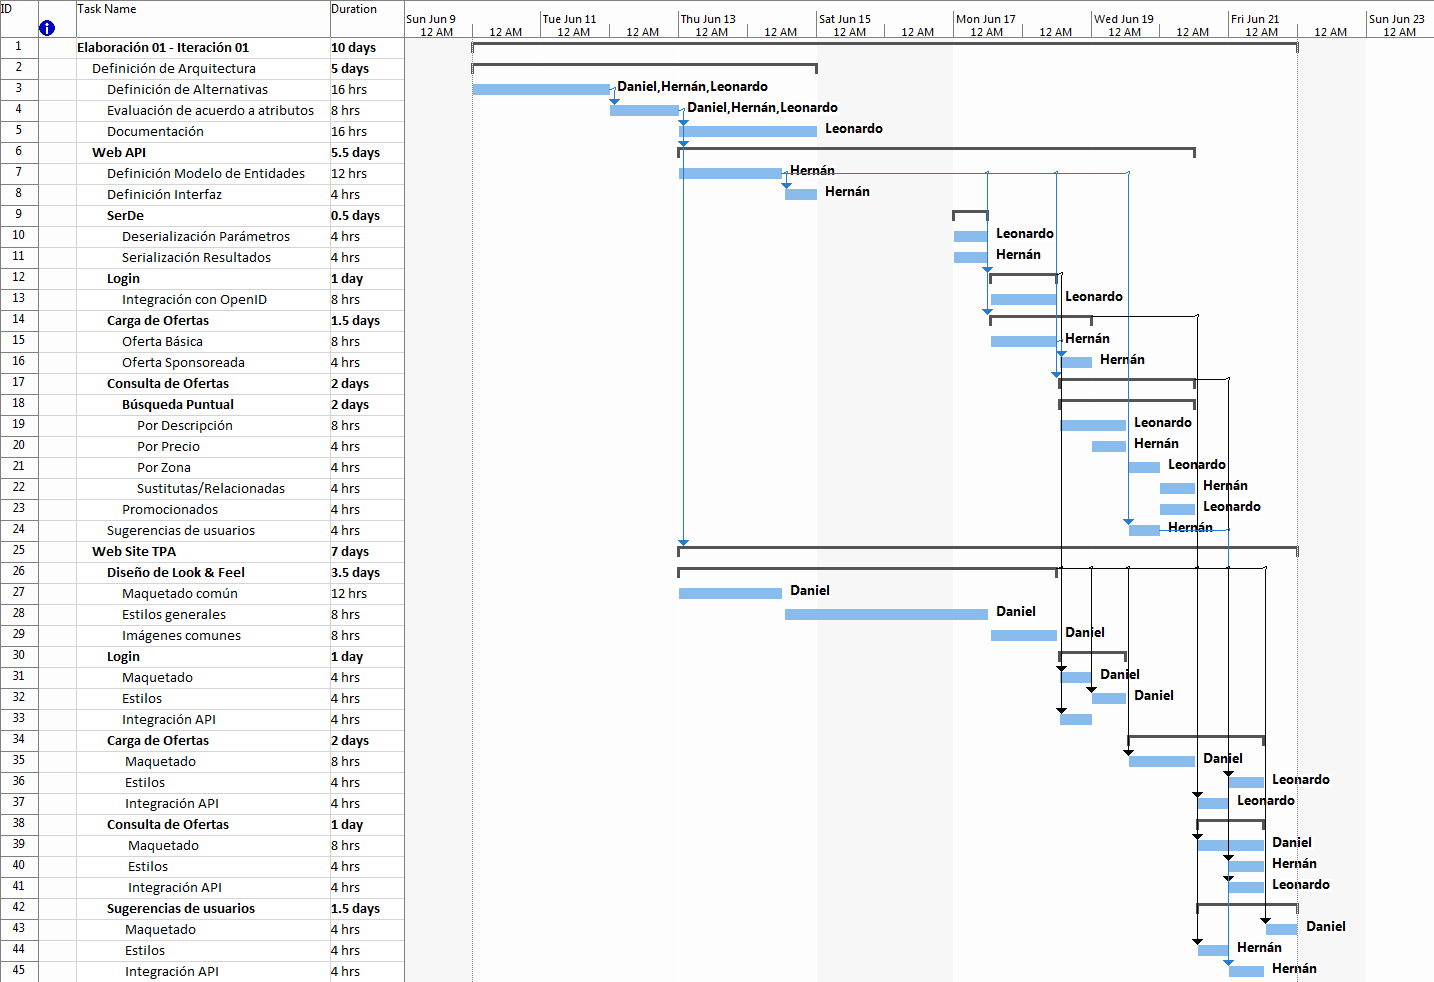
\includegraphics[height=0.75\textheight,angle=90]{TP2Planificacion}
\caption{Diagrama de Gantt de tareas de la primera iteraci\'on, con divisi\'on de tareas y asignaci\'on de recursos}
\label{fig:gantt}
\end{figure}


\section{Parte II}

 En esta segunda parte del informe presentamos el an\'alisis realizado al respecto de los distintos atributos de calidad identificados, exponiendo varios escenarios para cada uno de \'estos. Tambi\'en mostramos la arquitectura definida para la aplicaci\'on, utilizando distintos diagramas (de conectores y componentes, y de alocaci\'on), y complementamos estos \'ultimos mediante una descripci\'on detallada de la interacci\'on entre los distintos componentes y artefactos. Tambi\'en explicamos las decisiones que nos llevaron a definir la arquitectura, y c\'omo \'esta cubre los distintos escenarios de calidad.
 
 Por \'ultimo, compartimos nuestra apreciaci\'on al respecto de las similitudes y diferencias entre la modalidad de trabajo para el primer trabajo pr\'actico y \'este, comparando metodolog\'ias y alcances.
 

\section*{Atributos de Calidad y Escenarios}

\begin{escenario}{Usabilidad - Aprender a usar el sistema}{Que Todos y Todas lo puedan usar}
\fuente{Usuario}
\estimulo{Desea realizar por primera vez una consulta simple (ofertas de un producto o cercanas a una direcci\'on)}\artefacto{Sistema}
\entorno{En ejecuci\'on}
\respuesta{Realiza la consulta sin inconvenientes }
\medida{Realiza la consulta en menos de 30 segundos}
\end{escenario}

\begin{escenario}{Usabilidad - Usar sistema eficientemente}{Los usuarios contar\'an con un sistema de confianza configurable} 
\fuente{Usuario}
\estimulo{Desea agregar un \'item a su listado de confianza personal}
\artefacto{Sistema}
\entorno{En ejecuci\'on}
\respuesta{El \'item es configurado exitosamente en la posici\'on indicada de la lista}
\medida{El \'item se agrega en menos de 2 minutos}
\end{escenario}

\begin{escenario}{Usabilidad - Minimizar errores del usuario}{El sistema debe tener la capacidad de anticiparse a las b\'usquedas de los usuarios} 
\fuente{Usuario}
\estimulo{Desea ingresar bien el producto o direcci\'on}
\artefacto{Sistema}
\entorno{En ejecuci\'on}
\respuesta{Se sugieren valores para el producto o direcci\'on en base a valores aceptados por el sistema}
\medida{Las sugerencias aparecen en menos de 1 s. de ingresar una letra}
\end{escenario}

\begin{escenario}{Usabilidad - Personalizar sistema}{El sistema tendr\'a un mecanismo interno de reputaci\'on} 
\fuente{Usuario}
\estimulo{Desea asignar confiabilidad a un usuario u oferta}
\artefacto{Sistema}
\entorno{En ejecuci\'on} 
\respuesta{Se asigna la confiabilidad solicitada por el usuario }
\medida{El usuario encuentra satisfactorio poder personalizar la configuraci\'on de confianza}
\end{escenario}

%\begin{escenario}{}{Feedback}\fuente{Usuario}\estimulo{Desea dar feedback sobre la funcionalidad de b\'usqueda, y la ayuda provista para esta por el sistema}\artefacto{Sistema}\entorno{En ejecucion}\respuesta{Se registra el feedback del usuario }\medida{Tiempo entre la publicacion de la funcionalidad/mejora y el feedback de usuario.\end{escenario}

\begin{escenario}{Rendimiento}{Una caracter\'istica distintiva del sistema debe ser su inmediata respuesta} 
\fuente{Usuarios}  
\estimulo{Realiza consulta sobre ofertas de un producto}
\artefacto{Sistema}   
\entorno{Modo normal}  
\respuesta{El sistema procesa la consulta y obtiene el listado de ofertas acuerdo a la confianza personal del usuario}
\medida{El pedido es procesado en promedio en menos de 2 segundos}
\end{escenario}

\begin{escenario}{Rendimiento}{La actualizaci\'on de la informaci\'on debe realizarse al momento de realizarse su publicaci\'on} 
\fuente{Usuarios}  
\estimulo{Se env\'ia una oferta}
\artefacto{Sistema}   
\entorno{Modo normal}  
\respuesta{El sistema ingresa la oferta al repositorio de ofertas}
\medida{La oferta es tenida en cuenta en promedio 5 segundos despu\'es de enviada la informaci\'on al sistema}
\end{escenario}

\begin{escenario}{Rendimiento}{Las ofertas deben poder visualizase en un mapa}
\fuente{Usuarios} 
\estimulo{Solicita visualizar el resultado de una consulta en un mapa} 
\artefacto{Sistema}   
\entorno{Sistema sobrecargado}  
\respuesta{El sistema ingresa las ofertas en el mapa y env\'ia el mapa al usuario}
\medida{El pedido es procesado en promedio en menos de 10 segundos}
\end{escenario}

\begin{escenario}{Disponibilidad}{Tiempo de disponibilidad} 
	\fuente{Usuario} 
	\estimulo{Realiza una consulta de ofertas}
	\artefacto{Sistema}
	\entorno{Normal}
	\respuesta{El sistema responde a la consulta}
	\medida{El sistema devuelva la informaci\'on el 99,9\% de las veces}
\end{escenario}

\begin{escenario}{Disponibilidad}{Es posible utilizar el sistema sin conexi\'on}
	\fuente{Usuario} 
	\estimulo{Realiza consulta / env\'ia oferta }
	\artefacto{Aplicaci\'on cliente}
	\entorno{Sin conectividad}
	\respuesta{El sistema guarda la operaci\'on para sincronizar cuando vuelva la conectividad. }\medida{Disponibilidad offline}
\end{escenario}

\begin{escenario}{Disponibilidad - Tiempo de Reparaci\'on}{El sistema no debe caerse} 
	\fuente{Nodo del cluster}
	\estimulo{Se invalida, queda inutilizado}
	\artefacto{Sistema}
	\entorno{Normal}
	\respuesta{El sistema se adapta a los n-1 nodos, si fuera un nodo distinguido reasigna esta responsabilidad en otro nodo que se encuentre online. }
	\medida{El sistema se adapta en menos de 1 minuto desde la detecci\'on de la ca\'ida. Se detecta la ca\'ida en menos de 30 segundos.}
\end{escenario}

\begin{escenario}{Modificabilidad - Interoperabilidad}{Interactibilidad con redes sociales}
\fuente{Desarrollador}
\estimulo{Integrar el sistema con una nueva red social}
\artefacto{Sistema}
\entorno{Desarrollo}
\respuesta{Interfaz modificada o nueva interfaz para integrar con red social}
\medida{El esfuerzo de desarrollo es menor a 40 horas}
\end{escenario}

\begin{escenario}{Modificabilidad - Modularidad}{SpamBust ser\'a reemplazado por una m\'odulo propio} 
\fuente{Desarrollador} 
\estimulo{Intercambiar Spambust por implementaci\'on propia} 
\artefacto{Sistema} 
\entorno{Desarrollo} 
\respuesta{Intercambio de implementaci\'on de interfaz (inyecci\'on de nueva dependencia)} 
\medida{El esfuerzo de desarrollo es menor a 8 horas}
\end{escenario}

\begin{escenario}{Modificabilidad - Portabilidad}{Interacci\'on con usuarios de m\'ultiples plataformas}
\fuente{Desarrollador}
\estimulo{Adaptar interfaz web a un tipo de dispositivo nuevo }
\artefacto{Interfaz de usuario web }
\entorno{Desarrollo}
\respuesta{Adapta exitosamente la interfaz }
\medida{El esfuerzo de es menor a 40 horas}
\end{escenario}

\begin{escenario}{Modificabilidad - Capacidad}{El sistema debe ser r\'apido y se cuenta con computadoras de escritorio}
\fuente{Administrador del sistema}
\estimulo{Agregar un nodo al cluster}
\artefacto{Sistema }
\entorno{En ejecuci\'on}
\respuesta{El nodo se agrega y comienza a procesar exitosamente}
\medida{El nodo est\'a operativo en menos 2 horas}
\end{escenario}

\begin{escenario}{Modificabilidad - Content Management}{La aplicaci\'on deber\'a recomendar productos. Las reglas se cambiar\'an con frecuencia.} 
\fuente{Administrador de configuraci\'on}
\estimulo{Modifica relaci\'on entre productos}
\artefacto{Modulo de sugerencias}
\entorno{En ejecuci\'on}
\respuesta{El sistema utiliza la nueva configuraci\'on para relacionar productos a sugerir} 
\medida{La modificaci\'on demora menos de 2 minutos}
\end{escenario}

\begin{escenario}{Seguridad - Auditor\'ia}{Se deben poder anular ofertas y las asociaciones de consumidores quieren poder ver cu\'ales fueron} 
\fuente{Administrador de configuraci\'on}
\estimulo{Anular oferta} 
\artefacto{Sistema} 
\entorno{En ejecuci\'on} 
\respuesta{El sistema audita la anulaci\'on} 
\medida{Se identifica con una probabilidad mayor al 99\% al responsable de la modificaci\'on.}
\end{escenario}

\begin{escenario}{Calidad de datos}{Se quiere detectar spam/ofertas falsas} 
\fuente{Usuarios}
\estimulo{Env\'ian ofertas spam}
\artefacto{Detector de Spam}
\entorno{En ejecuci\'on }
\respuesta{El sistema marca las ofertas como spam. }
\medida{El sistema detecta spam con un 95\% de probabilidad.}
\end{escenario}

\begin{escenario}{Calidad de datos}{Se quiere detectar spammers/usuarios que informan ofertas falsas} 
\fuente{Confianza de usuario}
\estimulo{Supera el threshold de confianza}
\artefacto{ Sistema }
\entorno{En ejecuci\'on }
\respuesta{El sistema marca al usuario como spammer y lo blacklistea } 
\medida{Los usuarios sin confianza se detectan con probabilidad del 90\%}
\end{escenario}

\begin{escenario}{Seguridad - Autenticaci\'on (Assurance)}{Los usuarios podr\'an autenticarse usando OpenId}
\fuente{Usuario}
\estimulo{Se autentica}
\artefacto{Sistema}
\entorno{En ejecuci\'on}
\respuesta{El sistema valida las credenciales de usuario.}
\medida{El sistema resiste ataques de fuerza bruta sobre las credenciales y ataques de MiTM mediante certificados.}
\end{escenario}

\begin{escenario}{Seguridad - Ataques/Disponibilidad}{El sistema no debe caerse, esto incluye ataques de DDoS}
\fuente{Atacante}
\estimulo{Denegaci\'on de servicio distribuido}
\artefacto{ Sistema }
\entorno{En ejecuci\'on }
\respuesta{El sistema informa de sobrecarga en el sistema an\'omala}
\medida{El sistema detecta el ataque en menos de 2 minutos (?)}
\end{escenario}

\section*{Explicaci\'on de la Arquitectura}

\subsection*{Diagrama de Componentes y Conectores}

\subsubsection*{Arquitectura Global}

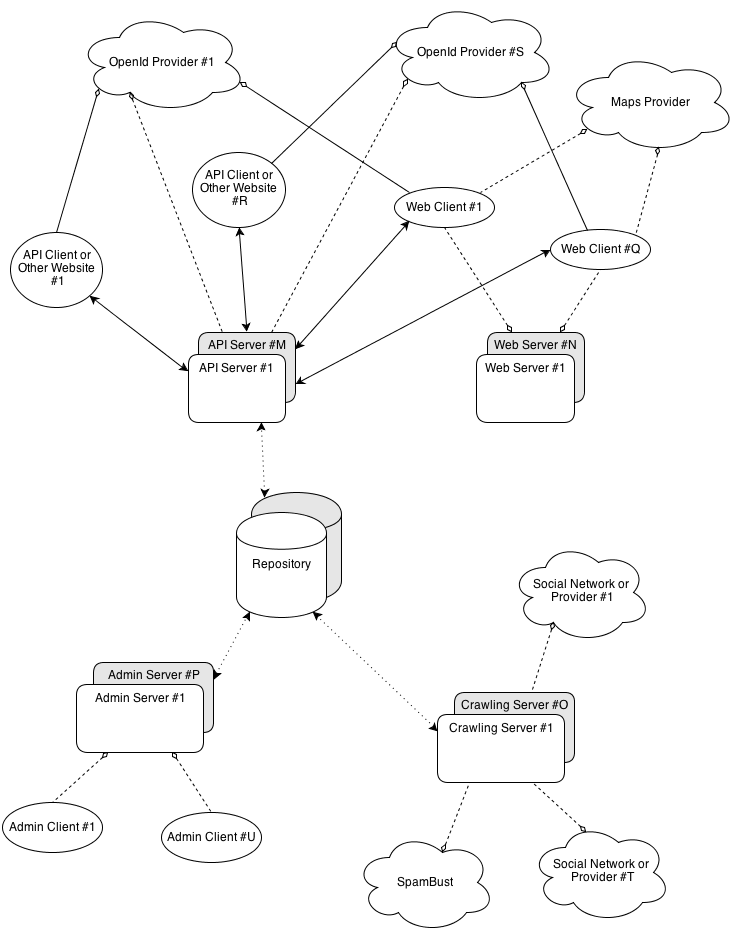
\includegraphics[scale=0.5]{ISW2_cNc_Global}


\subsubsection*{Consulta Web o API}

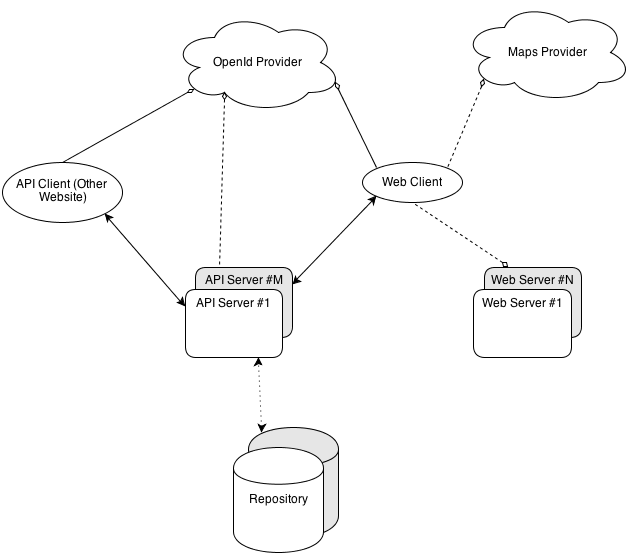
\includegraphics[scale=0.5]{ISW2_cNc_Consulta}

En el diagrama de la consulta web se identifican dos tipos de clientes, que son los clientes del sitio Web y los que consumen \'unicamente la API web. Tenemos tambi\'en dos tipos de componenetes servidor propios, que son los servidores del sitio Web y el servidores de la API web. Adem\'as, el diagrama nos muestra el repositorio de datos de configuraci\'on y consulta. Por \'ultimo, tenemos distintos tipos de servicios externos que son consumidos por los componentes anteriores, como son los proveedores de OpenId y el proveedor de mapas.

Los clientes Web consumen el contenido est\'atico directamente de los servidores del sitio Web, como puede ser el contenido HTML, JS, CSS e im\'agenes; se puede ver que el conector es de tipo cliente/servidor, lo que representa la sesi\'on que arma el navegador con el servidor, y el bloqueo del thread de UI principal entre sucesivos requests (GET principalmente). En principio, este tipo de interacci\'on es lo m\'as simple posible, sin nig\'un tipo de autenticaci\'on; la mayor parte del contenido es cacheable y compone la UI de la aplicaci\'on (no tiene datos sensibles).

Tanto los clientes Web como los clientes de la API (como pueden ser otros sitios web) interact\'uan con el componente servidor API.

La autenticaci\'on es resuelta como parte de esta interacci\'on, de acuerdo a la especificaci\'on de OpenId (\url{http://openid.net/specs/openid-authentication-2_0.html}):

\begin{itemize}
\item el cliente informa al componente servidor API el proveedor de OpenId que va a utilizar
\item el componente API establece una sesi\'on con el proveedor elgido (representamos esta sesi\'on con un conector de tipo cliente/servidor) que podr\'a ser reutilizada para subsiguientes validaciones o para obtener datos extra del mismo cliente
\item el cliente es redireccionado con el proveedor elegido para realizar la autenticaci\'on (representamos esta interacci\'on como un env\'io de un mensaje a trav\'es de una conexi\'on sincr\'onica)
\item el componente API reutiliza la sesi\'on establecida con el proveedor para verificar la informaci\'on de autenticaci\'on y para obtener datos adicionales
\end{itemize}

M\'as all\'a de manejar la autenticaci\'on, el componente servidor API responde a todos los pedidos de b\'usqueda o datos de configuraci\'on, de manera indistinta entre clientes Web o de API (usar\'ian el mismo puerto); el tipo de conexi\'on en este caso es asincr\'onica en ambos sentidos, para representar llamados tipo AJAX.

La interacci\'on con el proveedor de mapas asumimos que se puede resolver directamente desde el cliente, mediante alg\'un tipo de plugin descargado est\'aticamente desde el sitio Web.

El acceso al repositorio de datos y configuraci\'on lo hace \'unicamente el componente servidor API, para poder satisfacer los distintos requests, que agrupar\'ian todo el contenido din\'amico de la aplicaci\'on.

Por \'ultimo vale destacar que la cardinalidad del componente servidor API puede ser distinta a la del componente servidor Web, y dado que el primero atiende a consultas din\'amicas, con workflows m\'as complejos (como el de autenticaci\'on), y con mayor utilizaci\'on de recursos, podr\'ia ser necesario escalarlo en mayor medida que al segundo, que s\'olo responde a requests de contenido est\'atico. Adem\'as s\'olo es necesario implementar el proceso de autenticaci\'on en el componente servidor API, sustentado por el hecho de que s\'olo \'este tiene acceso al repositorio, simplificando la arquitectura.


\subsubsection*{Crawling de Redes Sociales y Sitios Web}

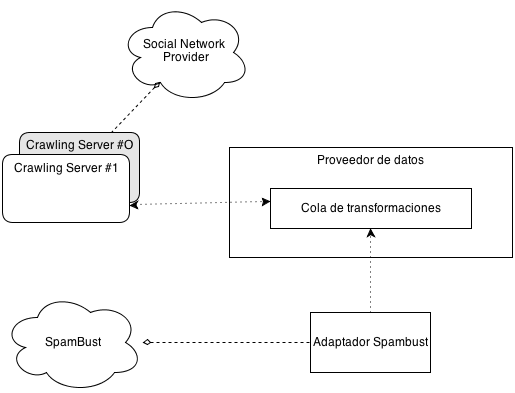
\includegraphics[scale=0.5]{ISW2_cNc_Crawling}

En el diagrama de crawling se identifica el componente de Crawling, el servicio de SpamBust, y el proveedor de red social (o sitio web de proveedor). Nuevamente, el diagrama nos muestra el repositorio de datos de configuraci\'on y consulta.

Los componentes de Crawling utilizan las distintas APIs provistas por las redes sociales para hacer las b\'usquedas de productos y ofertas; representamos esta interacci\'on mediante un conector de tipo cliente/servidor, para generalizar el comportamiento de las distintas APIs. Podemos tener distintos componentes de Crawling, trabajando de manera independiente, cada uno realizando b\'usquedas distintas sobre la misma red social, o a distintas redes sociales.

El servicio de SpamBust es utilizado por los componentes de Crawling para filtrar ofertas de dudosa integridad, o que provienen de usuarios con baja reputaci\'on. Esta interacci\'on tambi\'en es representada mediante un conector tipo cliente/servidor, para generalizar las posibles implementaciones.

Por \'ultimo, el repositorio es utilizado para consultar configuraci\'on de proveedores, usuarios, y redes sociales, y tambi\'en para persistir todos los datos de ofertas obtenidos en el proceso de crawling.


\subsubsection*{Administraci\'on}

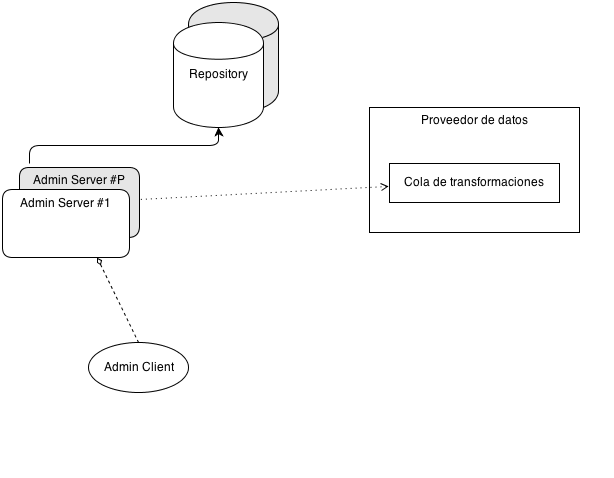
\includegraphics[scale=0.5]{ISW2_cNc_Administracion}

En el diagrama se identifican los componentes servidor y cliente de Administraci\'on. Adem\'as, el diagrama nos muestra el repositorio de datos de configuraci\'on.

El componente servidor de Administraci\'on provee tanto la UI como el contenido din\'amico de la aplicaci\'on de adminsitraci\'on, que se utiliza para el ABM de proveedores, publicidad, y otras variables que puedan afectar el comportamiento de la aplicaci\'on. Adem\'as, maneja un esquema de autenticaci\'on y autorizaci\'on propio, independiente de la aplicaci\'on principal, ya que la administraci\'on es realizada por usuarios internos. El acceso del componente cliente a la aplicaci\'on de adminitraci\'on se representa mediante un conector de tipo cliente/servidor.

Por \'ultimo, el repositorio es utilizado para persistir toda la informaci\'on de configuraci\'on, para ser utilizada por el resto de los sistemas.




\subsection*{Diagrama de Alocaci\'on}




\subsection*{Arquitectura y Calidad}

La arquitectura descripta en las secciones anteriores fue definida para cubrir los distintos escenarios detallados al comienzo del informe, y as\'i cumplir con los atributos de calidad identificados.

Desde el punto de vista de usabilidad, el mayor aporte de la arquitectura es la separaci\'on total de la interfaz de usuario. Esto permite, en gran medida, independizar caracter\'isticas de la UI que inciden directamente en la experiencia de usuario, como puede ser el maquetado.

Esta mayor independencia en el desarrollo de la UI nos ofrece varias ventajas:

\begin{itemize}
\item proveer distintas vistas que se adapten mejor a las preferencias del usuario, atacando temas como el uso eficiente, la personalizaci\'on, y la sensaci\'on de confort
\item ofrecer contenido est\'atico de ayuda para toda la UI, accesible r\'apidamente y cacheable, cubriendo necesidades como el aprendizaje del sistema
\item incluir validaciones simples y complejas del lado de cliente, minimizando la posibilidad de errores
\end{itemize}

Otro aspecto que aporta a la adaptabilidad y personalizaci\'on, es el soporte de la arquitectura para identificar usuarios y permitirles persistir configuraci\'on propia.

El siguiente atributo de calidad m\'as relevante, es el de rendimiento; en este caso la arquitectura lo ataca desde varios puntos. La arquitectura presenta varios componentes con responsabilidades diversas, y con bajo acoplamiento entre s\'i, facilitando partir las estrategias de performance entre todos estos componentes.

Desde el punto de vista de la experiencia de usuario, la arquitectura separa todos los request de contenido est\'atico, de los requests de contenido din\'amico, permitiendo paralelizar con distinta cardinalidad cada uno de esto puntos, destinando mayor cantidad de recursos a los componentes que m\'as lo requieren. 

En el caso de los componentes servidor API, se impulsa un aplicaci\'on stateless, en donde cada request tiene toda la informaci\'on necesaria para ser atendido (header de autenticaci\'on y par\'ametros), lo que permite repartirlos de acuerdo a una estrategia de cola predefinida (round robin, recursos disponibles, etc.), aumentando el throughput (y disminuyendo el delay al no saturar recursos). Al alocar componentes relacionados en el mismo recurso f\'isico, como una partici\'on del repositorio y un componente servidor API, se minimiza el tr\'afico de red para requests que se puedan responder con esa partici\'on, y as\'i tambi\'en el delay.

Desde el punto de vista de los componentes de crawling, se paraleliza el trabajo en distintos recursos f\'isicos, aumentando el throughput.

El atributo de integrabilidad/extensibilidad se cubre desde varios puntos:

\begin{itemize}
\item el bajo acoplamiento entre componentes, permite su f\'acil modificaci\'on, en particular si el cambio no requiere cambiar la interfaz, y a\'un en estos casos se puede recurrir al uso de patrones conocido como el de adapter, bridge, etc
\item la separaci\'on de la UI, da mayor flexibilidad a la hora de soportar nuevos dispositivos y plataformas
\item los componentes de Administraci\'on dan soporte a la capacidad del sistema de modificarse en tiempo de ejecuci\'on.
\item el acceso al servicio de SpamBust como un componente separado facilita el reemplazo de \'este por una implementaci\'on propia, mientras que se respete la interfaz
\item el escalamiento horizontal de recursos cr\'iticos, como el repositorio, permite adaptar su capacidad en tiempo de ejecuci\'on
\item el acceso a las redes sociales de manera agn\'ostica de la API (utilizando patrones como Adapter, etc), agiliza la incorporaci\'on de nuevas redes sociales y sus APIs
\end{itemize}
  
La arquitectura cubre los aspectos de disponibilidad ofreciendo redundancia en cada uno de los subsistemas.

En el caso de los componentes servidor Web y API, se ofrece alta disponibilidad paralelizando los requests entre varias instancias de \'estos, controlando activamente el estado de cada uno para detectar ca\'idas y redireccionar cuando sea necesario.

En cuanto al repositorio, adem\'as de escalar horizontalmente mediante nuevas particiones, ofrece redundancia activa para cada una de \'estas; desde el punto de vista de la alocaci\'on, esta redundancia va de la mano con la replicaci\'on de los otros componentes que conviven en el mismo recurso (como el servidor API).

Por \'ultimo, tanto el sistema de Crawling como los componentes de Administraci\'on ofrecen un esquema de alta disponibilidad, replic\'andose cada uno en varios recursos.

Respecto a los aspectos de seguridad y auditor\'ia, todo el acceso a contenido din\'amico se hace desde componentes que implementan un esquema estricto de autenticaci\'on, y en el caso de administraci\'on implementan tambi\'en un esquema de autorizaci\'on. Esto \'ultimo permite que todo acceso al repositorio est\'e acompa\~nado de credenciales que identifican al usuario responsable por el acceso, y as\'i poder auditar la interacci\'on.

Al separar la API de acceso p\'ublico de los componentes de Administraci\'on, podemos llevar la mayor parte de las operaciones de modificaci\'on de la aplicaci\'on a un ambiente privado y controlado, dejando en la API p\'ublica \'unicamente operaciones de consulta y de configuraci\'on personal del usuario.

Para finalizar, respecto a la calidad e integridad de datos, la arquitectura presenta un esquema modular para el intercambio del componente Spambust, de acuerdo a la evaluaci\'on de resultados; adem\'as \'este se encuentra conectado de una manera que lo acerca lo m\'as posible al origen de los datos, que es al momento de recolecci\'on.

\section*{Conclusi\'on}

Al momento de comparar las metodolog\'ias utilizadas para la primera y segunda parte, notamos c\'omo \'estas se ajustan a las caracter\'isticas de cada uno de los escenarios: tiempo de planeamiento, incorporaci\'on de cambios, dependencias entre los distintos hitos, los entregables esperables en cada etapa, cuan involucrado debe estar el cliente en el proceso de desarrollo. 

Puede verse que las m\'etodolog\'ias hacen foco en distintas cosas, Scrum hace foco en ir explorando el problema a medida que se lo va resolviendo y en los pedidos del momento del cliente. RUP por otro lado hace incapi\'e en el an\'alisis y planificaci\'on antes que otras tareas para resolver el problema.

Esto hace que en scrum haya una mayor visibilidad del avance hacia el cliente a fin de lograr su satisfacci\'on y adaptabilidad a los cambios en el negocio o necesidades del cliente, esto \'ultimo puede verse con el cambio de los stories dentro del backlog y en la selecci\'on de las mismas antes de comenzar un sprint. Por otra parte la manera que tiene esta metodolog\'ia agil para afrontar los problemas que pueden surgir es de alguna manera mediante las standup meetings diarias. 

En RUP lo que logra el foco en el an\'alisis y planificaci\'on es que pueda mitigarse (o al menos conocerse) que inconvenientes pudieran surgir, as\'i como ver la viabilidad de los requerimientos del cliente y en que cuestiones debe hacerse foco para satisfacer al mismo, esto \'ultimo utilizando los escenarios de calidad. Dado que la metodolog\'ia permite planificar el proyecto por entero es posible de alguna manera estimar su costo, lo cual en organizaciones que manejan prespuestos anuales puede ser sumamente \'util a la hora de seleccionar proyectos.

Entendemos que estas dos metodolog\'ias si bien pueden considerarse como \"rivales\", podr\'ian verse como complementarias. RUP podr\'ia utilizarse para el an\'alisis macro de un proyecto, para poder entender el problema y diseñar su arquitectura, y scrum para en el desarrollo de los distintos módulos que componen la arquitectura generada, benefici\'andose as\'i el proyecto de la adaptabilidad a los cambios que pudieran surgir a posteriori en el negocio.




\end{document}
